
\chapter{Evaluation}
% \section{Metric Based Analysis}
% \section{Visual Based Analysis}
In line with the research questions, the evaluation section aims to quantify the performance gains obtained by using the Proxy Attention method. The section will compare the performance of networks that were trained with, and without Proxy Attention on the basis of classification metrics, and explainability improvements. 

Note that complete performance logs can be found in the appendix.
\section{Accuracy}
This section explores the validation accuracy obtained by the models for different hyperparameters and datasets. Since the task at hand is a classification task, this measure is a direct comparison of the performance of the models.

\section{Explanability}
This section explores the explainability of the models for different hyperparameters and datasets by using a trained model to generate attention maps for a given input image. The attention maps are compared between the same network (with the same hyperparameters) trained with and without Proxy Attention.

% \begin{figure}[h]
%     \centering
%     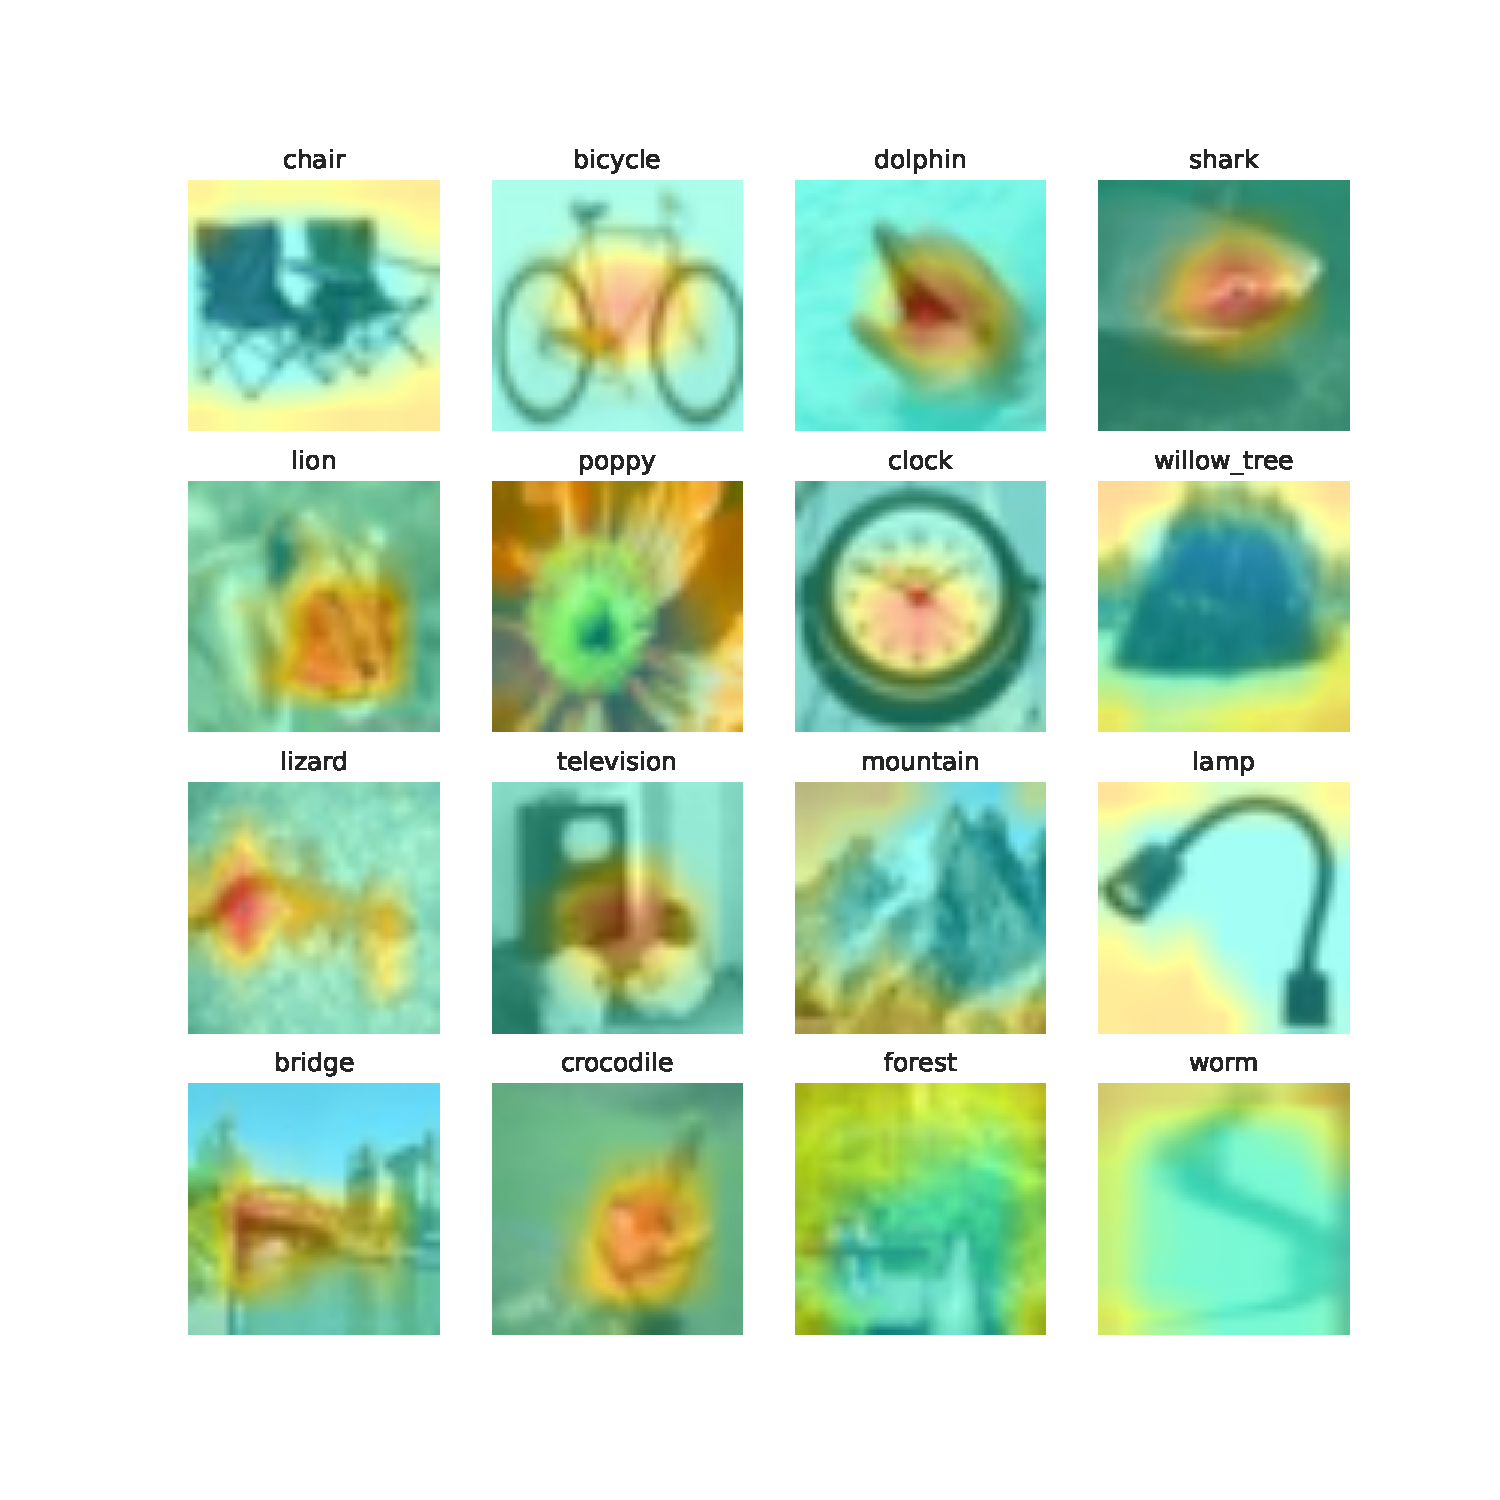
\includegraphics[width=0.8\textwidth]{images/proxy.pdf}
% 	\caption{}
%     \label{fig:thresholds}
% \end{figure}

% figure with two subfigures
\begin{figure}[h]
    \centering
    \begin{subfigure}[b]{0.7\textwidth}
        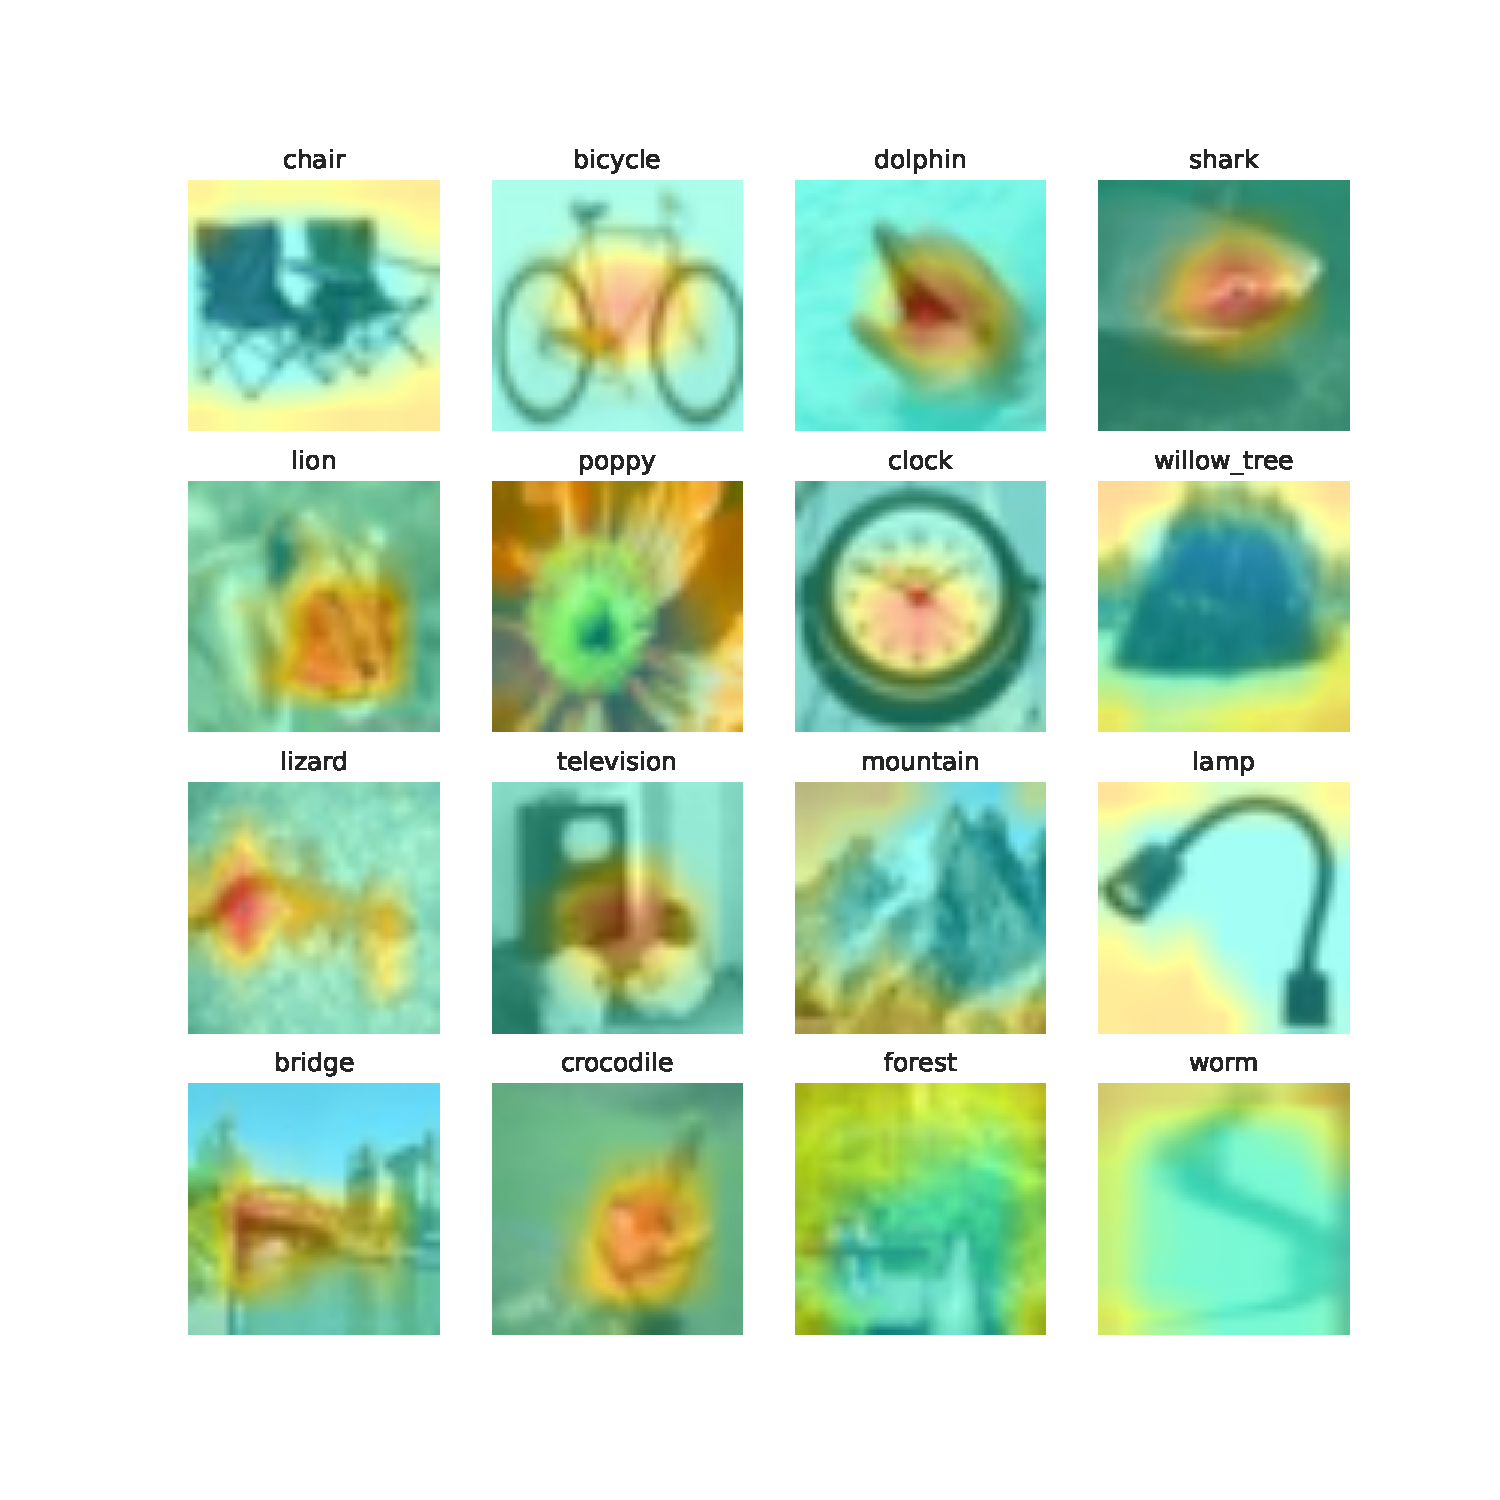
\includegraphics[width=\textwidth]{images/proxy.pdf}
        \caption{With Proxy Attention}
        \label{fig:proxy}
    \end{subfigure}
    \hfill
    \begin{subfigure}[b]{.7\textwidth}
        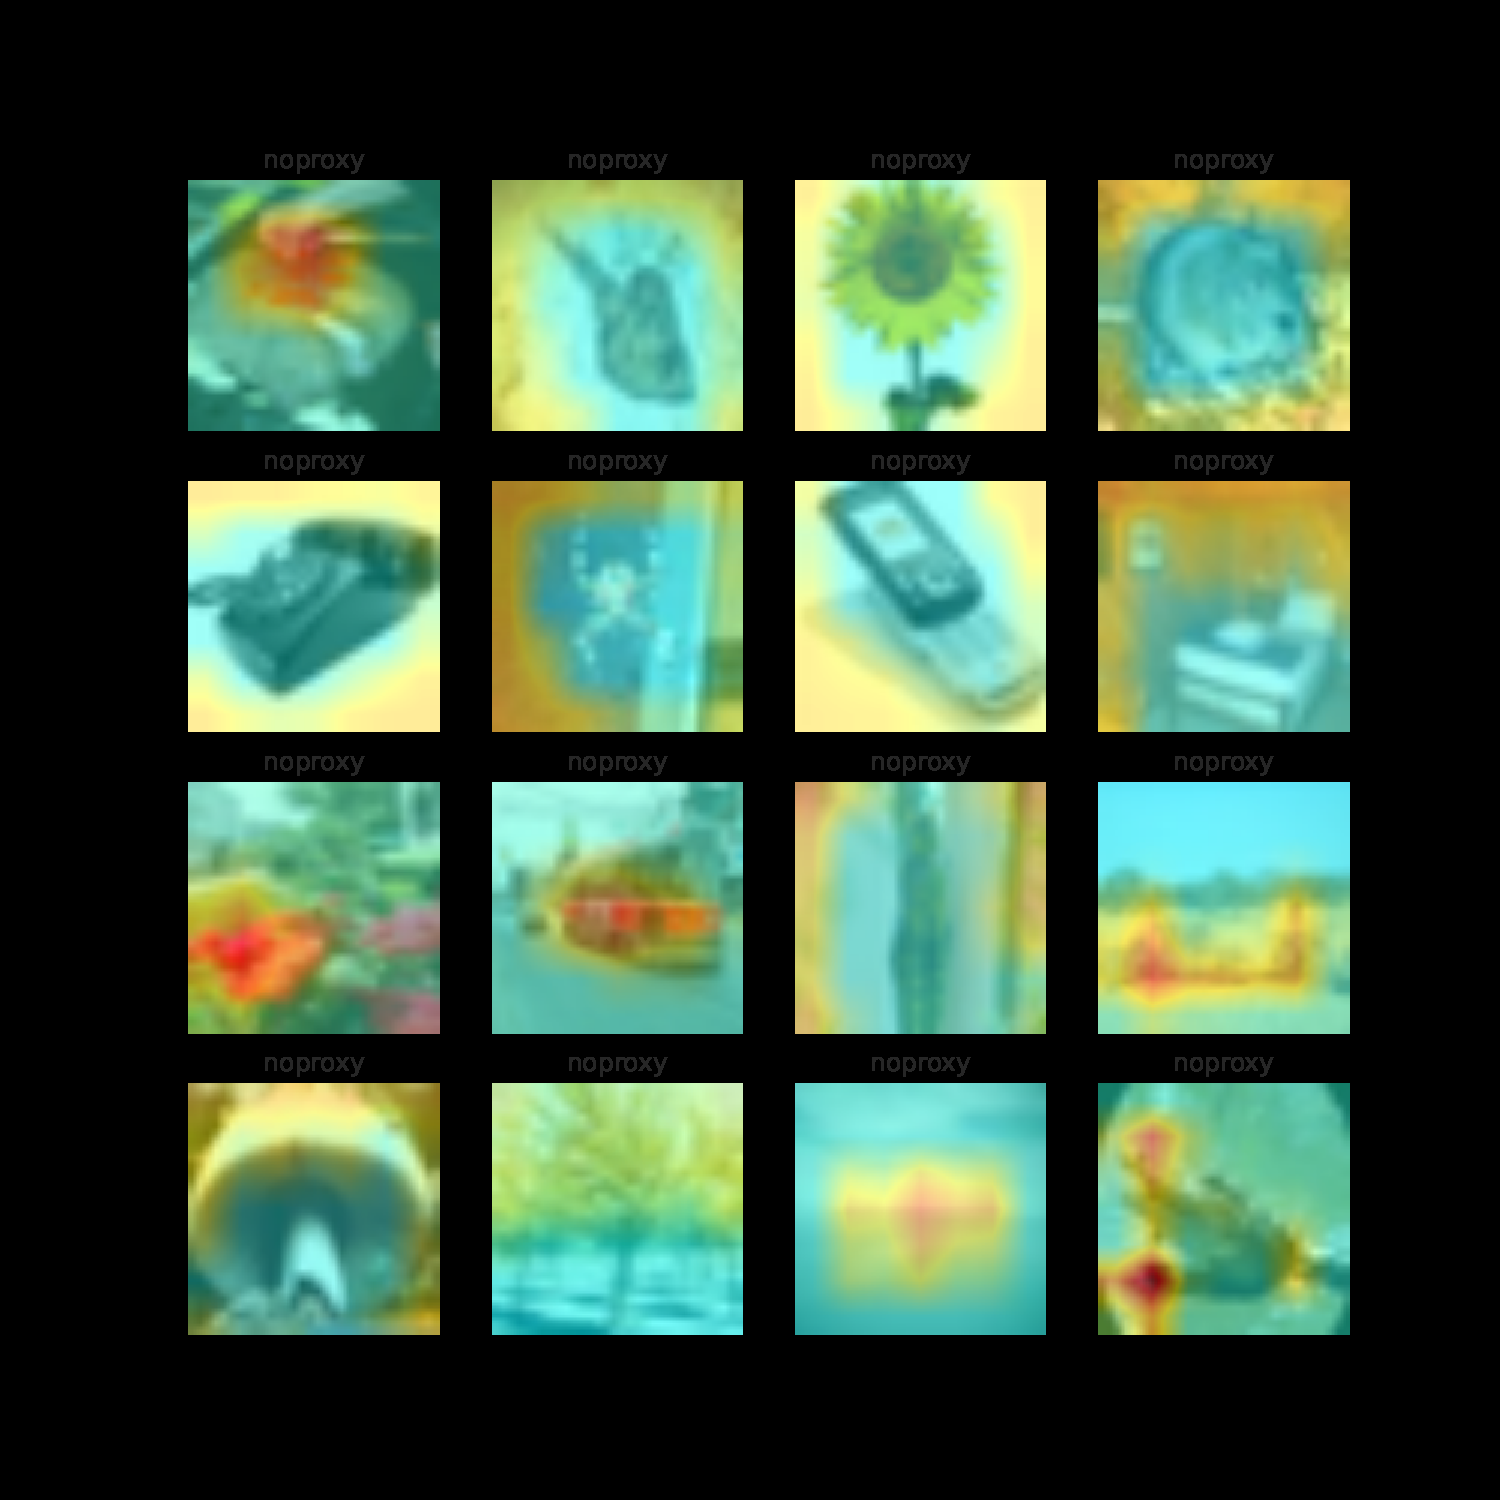
\includegraphics[width=\textwidth]{images/noproxy.pdf}
        \caption{Without Proxy Attention}
        \label{fig:noproxy}
    \end{subfigure}
    \caption{Comparison of attention maps generated by models trained with and without Proxy Attention}
    \label{fig:attention}
\end{figure}

\begin{figure}[h]
    \centering
    \begin{subfigure}[b]{0.7\textwidth}
        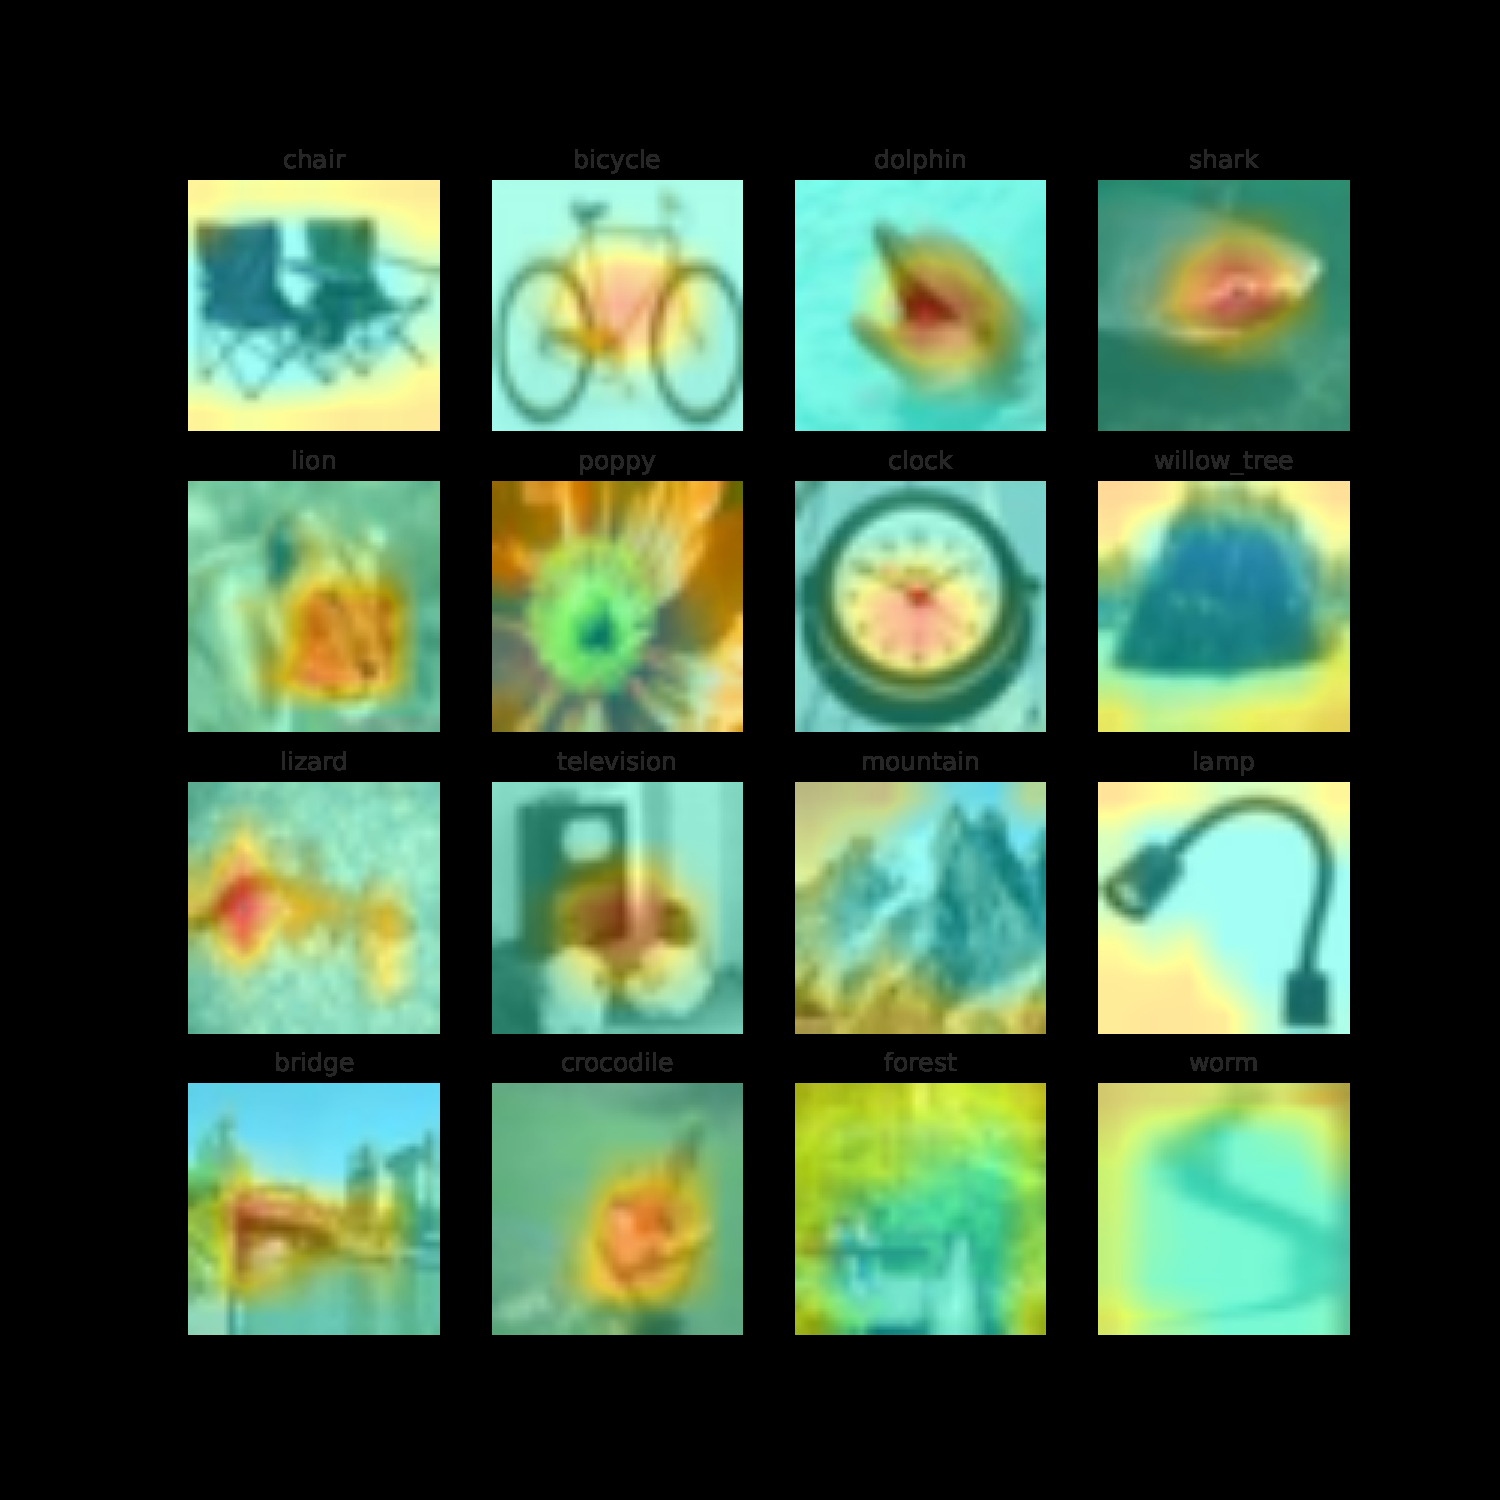
\includegraphics[width=\textwidth]{images/proxy_1.pdf}
        \caption{With Proxy Attention}
        \label{fig:proxy2}
    \end{subfigure}
    \hfill
    \begin{subfigure}[b]{.7\textwidth}
        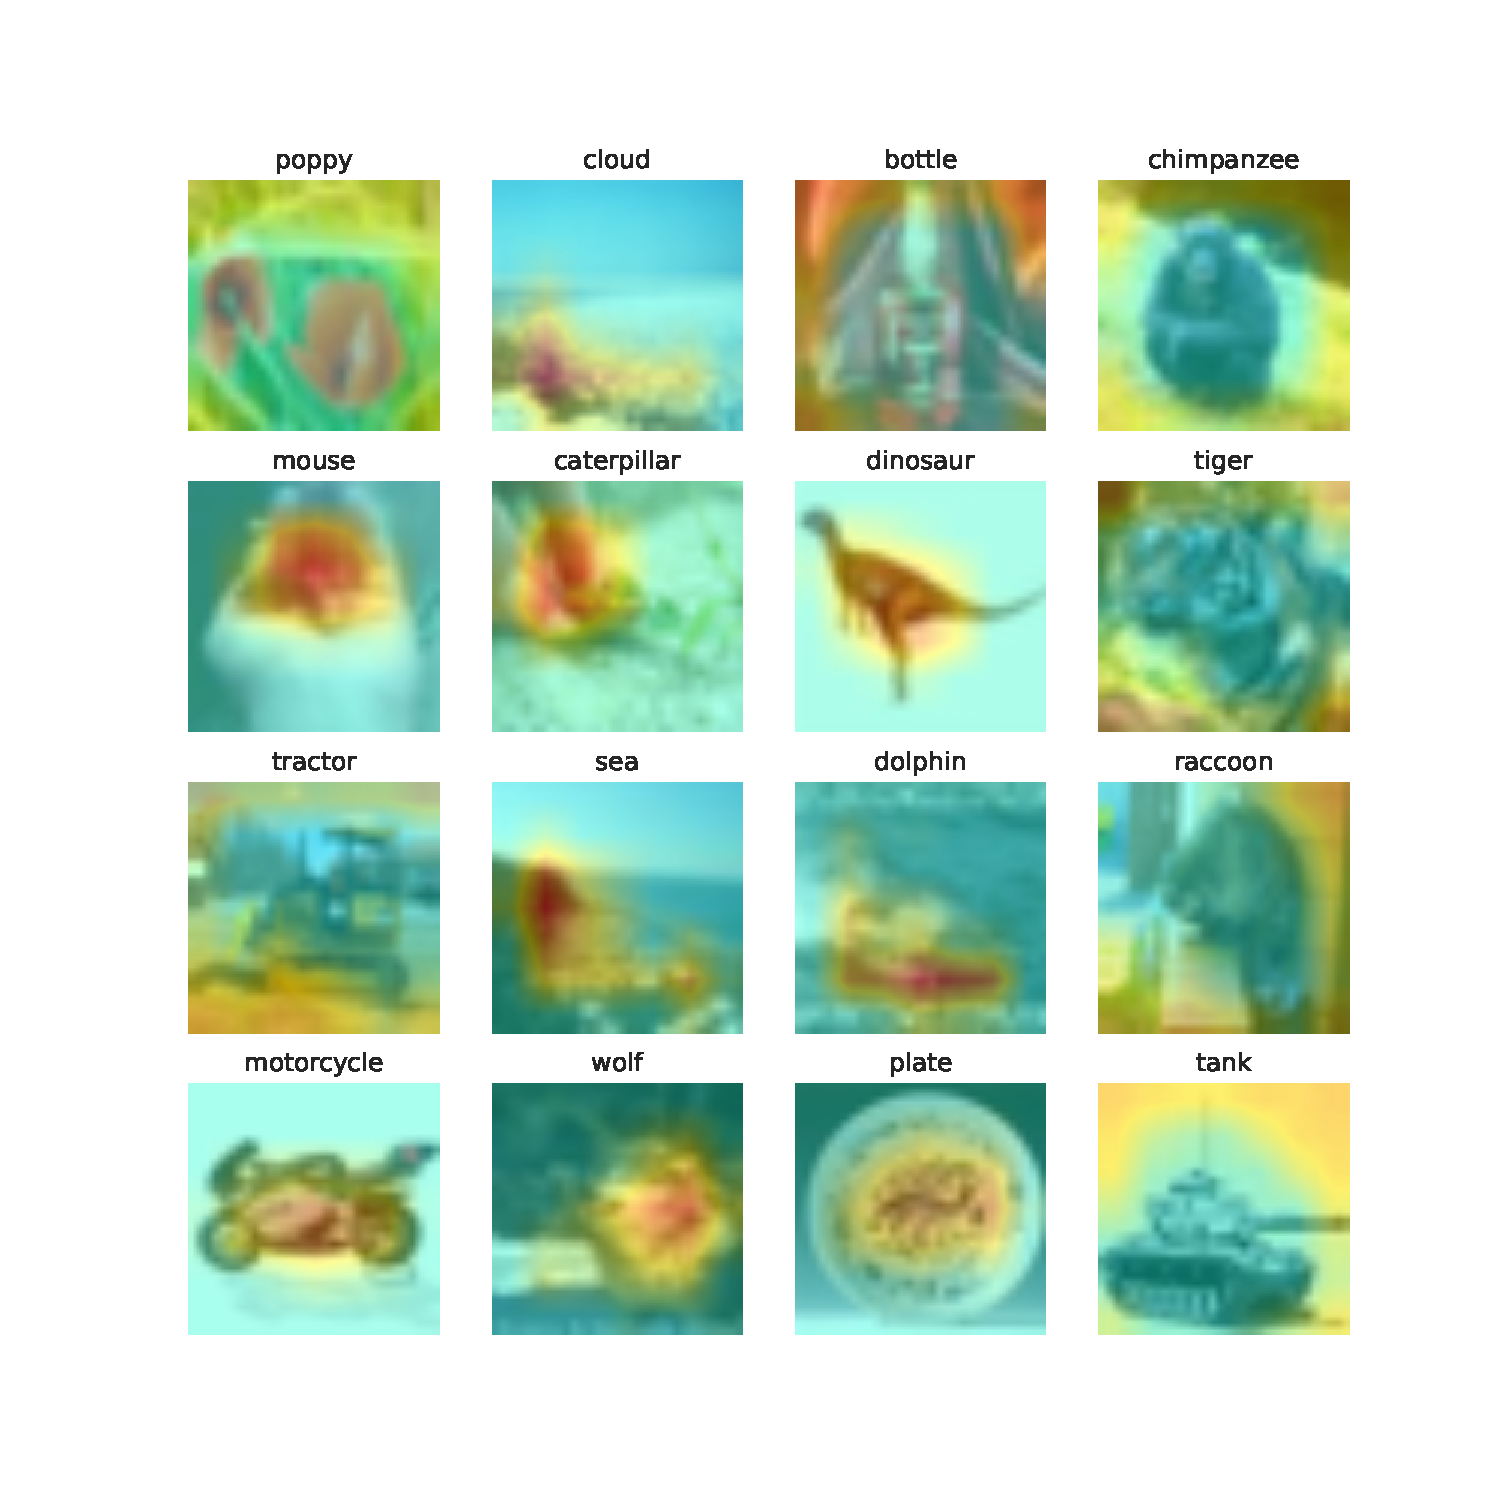
\includegraphics[width=\textwidth]{images/noproxy_1.pdf}
        \caption{Without Proxy Attention}
        \label{fig:noproxy2}
    \end{subfigure}
    \caption{Comparison of attention maps generated by models trained with and without Proxy Attention}
    \label{fig:attention2}
\end{figure}

\begin{figure}[h]
    \centering
    \begin{subfigure}[b]{0.7\textwidth}
        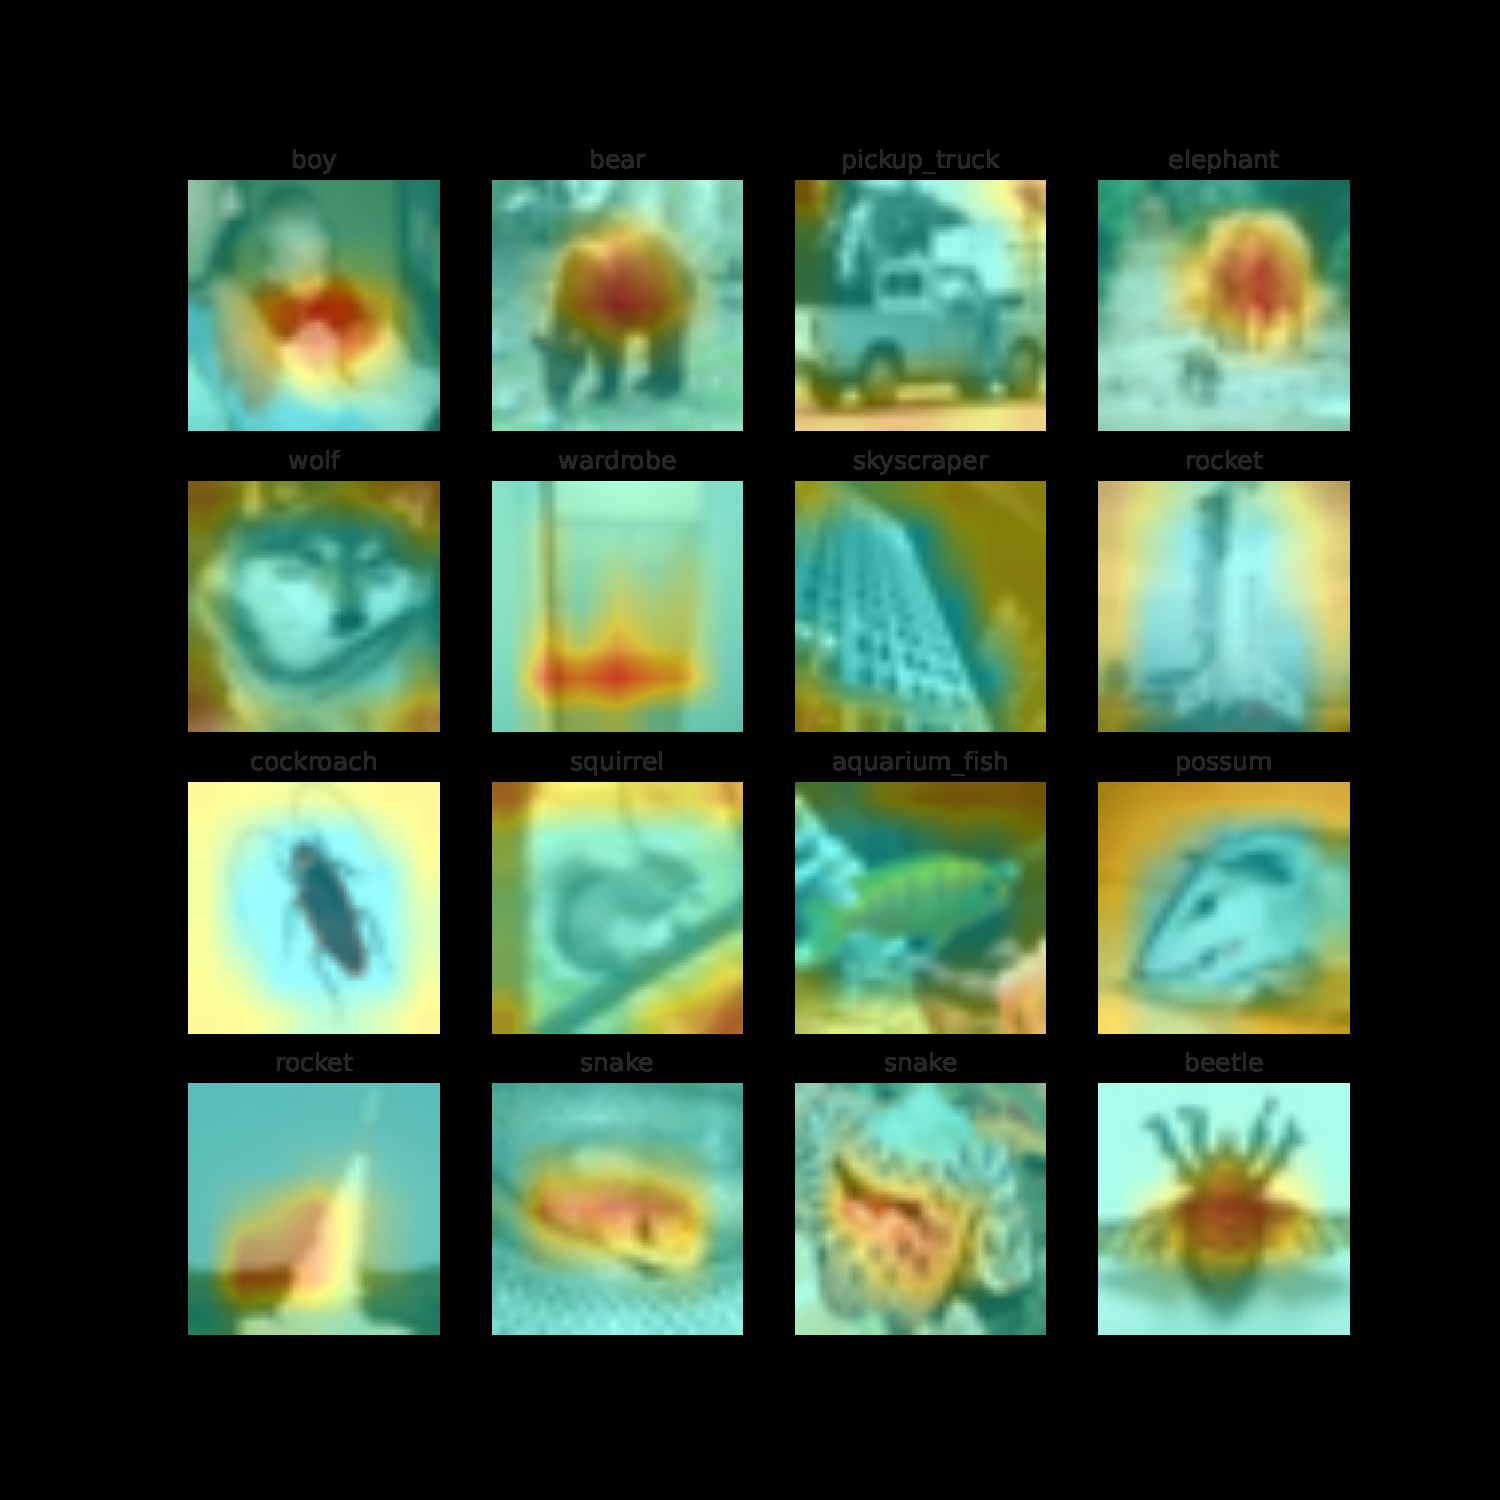
\includegraphics[width=\textwidth]{images/proxy_2.pdf}
        \caption{With Proxy Attention}
        \label{fig:proxy3}
    \end{subfigure}
    \hfill
    \begin{subfigure}[b]{.7\textwidth}
        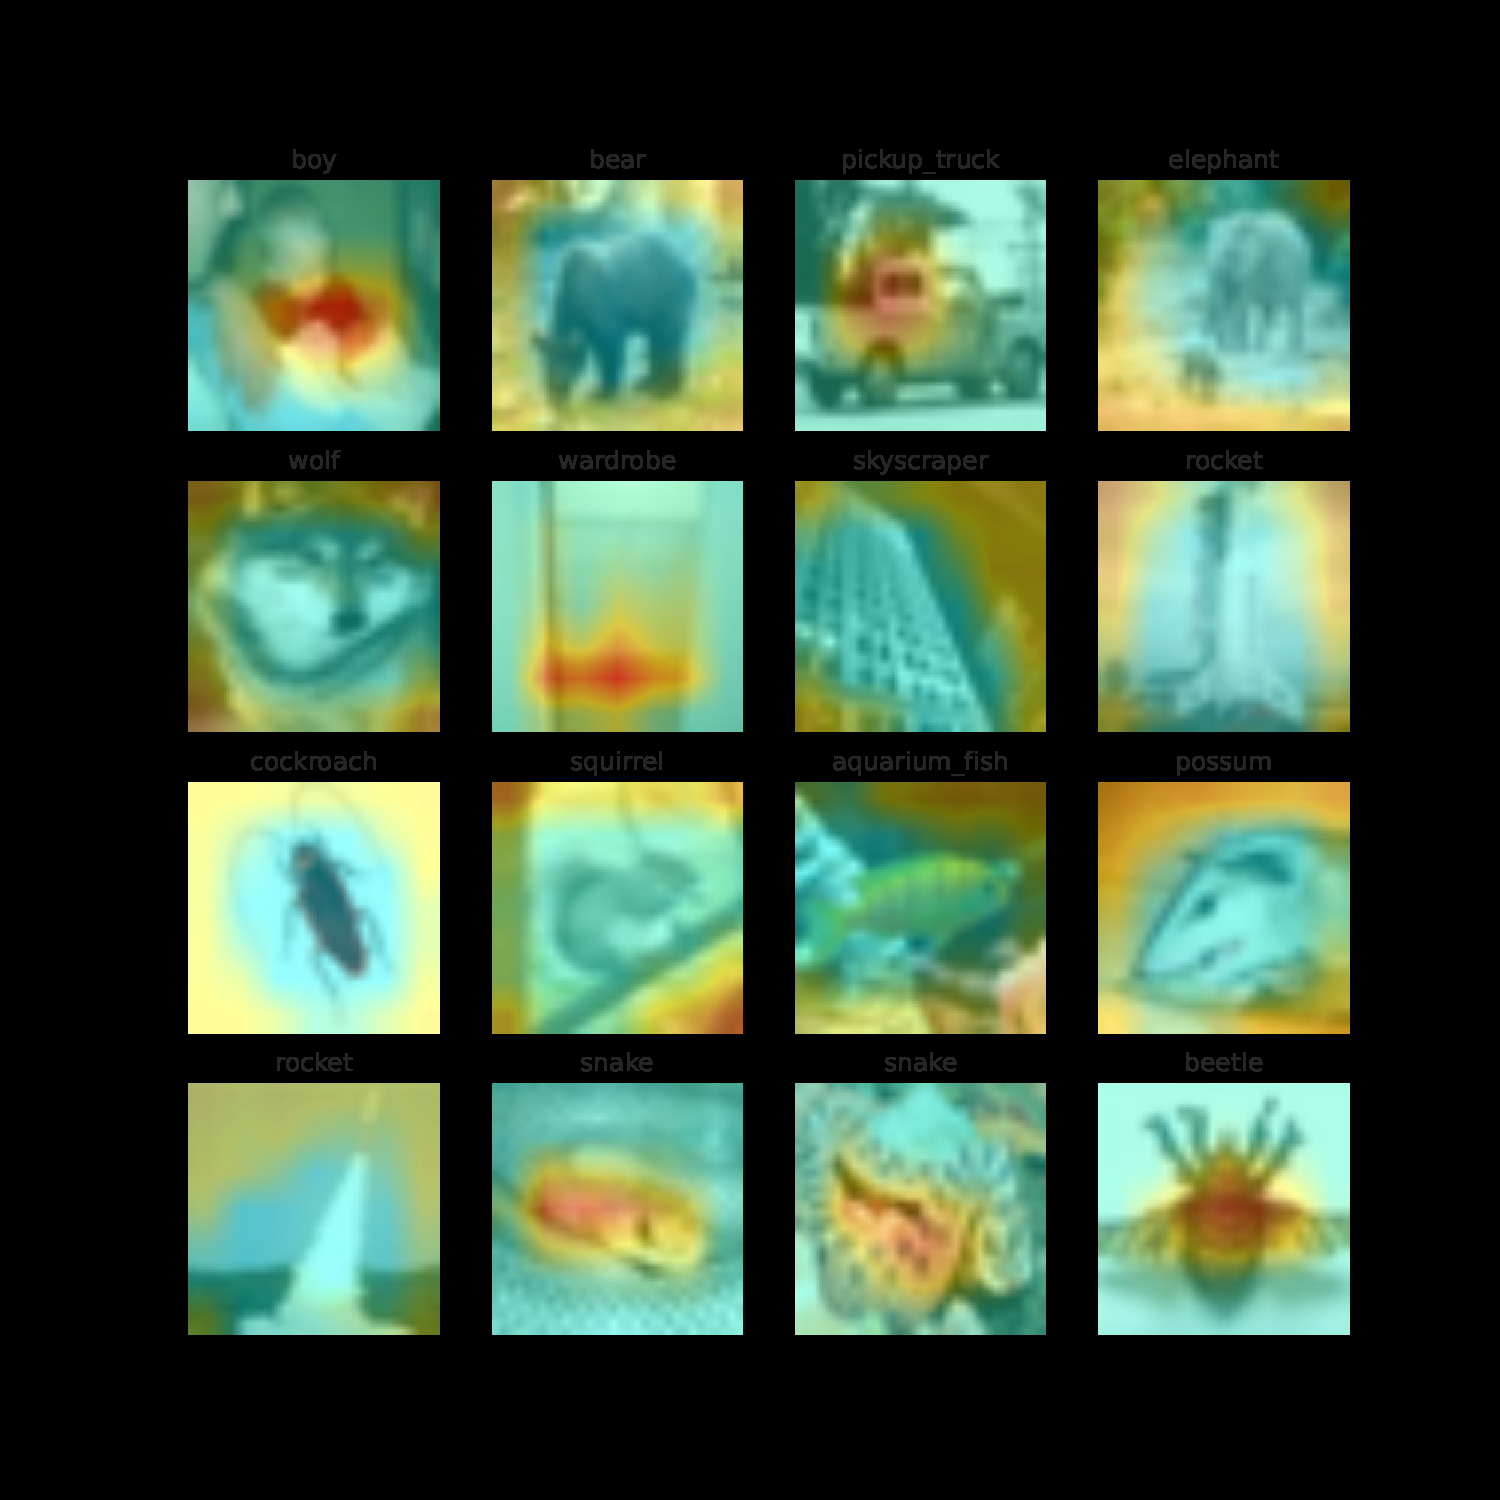
\includegraphics[width=\textwidth]{images/noproxy_2.pdf}
        \caption{Without Proxy Attention}
        \label{fig:noproxy3}
    \end{subfigure}
    \caption{Comparison of attention maps generated by models trained with and without Proxy Attention}
    \label{fig:attention3}
\end{figure}





\section{Summary}
